\section{Introduction}
This project proposes the use of biological signals, such as heart rate or muscle contractions, to generate musical signals.
The project aims to provide a standard Musical Instrument Digital Interface (MIDI) for artists and performers to use.
Additionally, the project aims to implement lighting control using the same biological signals to provide a novel interface for controlling lights.

\subsection{Background}
Music has been a form of human expression for over 40,000 years\cite{killin:2018}.
Throughout this time, the creation of music has relied on the skill and dexterity of artists
who have dedicated years to practicing in order to become proficient.
This has presented accessibility challenges for individuals who may be unable to physically perform such actions
or to those who do not have the time required to learn.
This project offers a solution to this challenge by providing a platform for creating music that can be accessible to everyone.
Additionally, this project allows for multifaceted performances due to the lack of physical restrictions on performers
during the dynamic creation of music.

This project is also beneficial to current artists as the addition of lighting control allows for more engaging performances.
Previously, lighting control has been done manually by a skilled lighting technician or automatically triggered by sound.
This project allows the lighting to be controlled directly by the performer, which could allow for much more compelling lighting setups.


A biosignal is a form of communication between biological systems\cite{semmlow:2018},
they are used in the body to detect various biological events such as muscle contractions and heartbeats\cite{escabí:2012}.
These signals can be detected using various types of sensors, including electric, mechanical, acoustic, and infrared sensors\cite{kaniusas:2012}.

A market analysis shows that there is a variety of research relating to the creation of music from biosignals.
Thies\cite{thies:2012} created real time game music control using biosignals.
Nerness\cite{Nerness:2019} created a musical stethophone.
Jaimovich researched both biosignal algorithms for musical application\cite{jaimovich:2015},
and sound interactions for biosignal and dancers\cite{Jaimovich:2016}.
However, while there has been research into controlling music with biosignals,
there is a research gap in controlling lighting with biosignals, which is what this project aims to fill.

\section{Project Objectives}
For this project to be successful, it is necessary to fulfill various requirements.
The requirements for this project are:

\begin{enumerate}
    \item The system must be composed of inexpensive parts
    \begin{enumerate}
        \item Sensors must fall within the allocated budget
        \item PCBs must use off the shelf, easily sourced components
        \item Components must be easily replaceable for minimal cost if something were to fail
    \end{enumerate}
    \item The system output must operate remotely to the acquired sensor data at a range of at least 30m
    \begin{enumerate}
        \item The acquisition of sensor data must be completely detached from the system output
        to allow for more complicated off-body setups
        \item The remote system must be compliant with ISO/IEC 15149-1:2014 or equivalent
        \item The wireless system must have a Packet Error Rate (PER) of no more than 1\%
        \item The wireless system must still be functional in a noisy environment
    \end{enumerate}
    \item The system must output MIDI messages
    \begin{enumerate}
        \item The MIDI output port must be IEC 63035:2017 compliant
        \item The system must also provide MIDI over USB for greater compatibility with newer devices
    \end{enumerate}
    \item The system must incorporate lighting control
\end{enumerate}

\section{Assumptions and Constraints}
Assumptions:
\begin{itemize}
    \item The users of the system have basic knowledge of music theory and performance.
    \item The system will be used in conjunction with a lighting console that maps all the fixture addresses correctly.
    \item The system will be used in an indoor environment with stable temperature and humidity.
    \item The performers will be able to wear biosignal sensors comfortably during their performance.
    \item The sweat from the performers will be mitigated to avoid short-circuiting the electrodes.
    \item The system will be operated by a skilled technician during live performances.
\end{itemize}

Constraints:
\begin{itemize}
    \item The total cost of the system cannot exceed \$600.
    \item The size and weight of the whole system must be compact enough to transport in a standard travel bag.
    \item The size and weight of the on-body subsystem must be wearable for several hours without fatigue.
    \item The system must be compatible with standard MIDI interfaces and protocols.
\end{itemize}

The given constraints are cost, size, weight, and compatibility.
The cost is a constraint because the budget of the project is separate to the \$600 allocated limit.
So, if the project goes over budget it may continue, but if it goes past the allocated limit, the project will not be able to continue.
The size and weight are constraints because the project needs to be portable enough to effectively use.
The system compatibility is a constraint because it is required for the system to correctly operate with other unknown systems.

\section{Scope}
In order to mitigate the risk of other concurrent projects running over scope, additional stretch goals have
been added to the scope of this project. The stretch goals allow for increasing in scope
while still strictly maintaining an achievable scope for this project.
A breakdown of the scope of this project can be found in \autoref{tab:scope}, \autoref{tab:scope_stretch}, and \autoref{tab:scope_out}.

\begin{table}[!ht]
    \caption{Project in-scope list}\label{tab:scope}
    \centering
        \begin{tabular}{|l|c|}
        \hline
        \multirow{2}{7em}{On-body Device}     & \cellcolor{green!25}Communication between sub-systems           \\ \cline{2-2}
        ~                                     & \cellcolor{green!25}Basic sensor reading                        \\ \hline \hline
        \multirow{2}{7em}{Lighting Control}   & \cellcolor{green!25}Lighting fixture control                    \\ \cline{2-2}
        ~                                     & \cellcolor{green!25}Test setup                                  \\ \hline \hline
        \multirow{3}{7em}{System Integration} & \cellcolor{green!25}Wireless communication                      \\ \cline{2-2}
        ~                                     & \cellcolor{green!25}Integration with music generation           \\ \cline{2-2}
        ~                                     & \cellcolor{green!25}Integration with lighting generation        \\ \hline
    \end{tabular}

\end{table}

\begin{table}[!ht]
    \caption{Project stretch-goal list}\label{tab:scope_stretch}
    \centering
        \begin{tabular}{|l|c|}
        \hline
        Sensors                               & \cellcolor{orange!25}Wearable sensor design             \\ \hline \hline
        \multirow{3}{7em}{MIDI}               & \cellcolor{orange!25}Compliant MIDI implementation      \\ \cline{2-2}
        ~                                     & \cellcolor{orange!25}MIDI timecode quantisation         \\ \cline{2-2}
        ~                                     & \cellcolor{orange!25}MIDI output timecode               \\ \hline \hline
        \multirow{4}{7em}{System Integration} & \cellcolor{orange!25}Performance application testing    \\ \cline{2-2}
        ~                                     & \cellcolor{orange!25}Bi-directional communication       \\ \cline{2-2}
        ~                                     & \cellcolor{orange!25}Real-time system tunability        \\ \cline{2-2}
        ~                                     & \cellcolor{orange!25}PCB housing design for main board  \\ \hline
    \end{tabular}

\end{table}

\begin{table}[!ht]
    \caption{Project out-of-scope list}\label{tab:scope_out}
    \centering
        \begin{tabular}{|l|c|}
        \hline
        Sensors                               & \cellcolor{red!25}Sensors as independent systems        \\ \hline \hline
        \multirow{2}{7em}{MIDI}               & \cellcolor{red!25}Wireless MIDI                         \\ \cline{2-2}
        ~                                     & \cellcolor{red!25}MIDI threshold points                 \\ \hline \hline
        Lighting Control                      & \cellcolor{red!25}Lighting controller input support     \\ \hline \hline
        \multirow{2}{7em}{System Integration} & \cellcolor{red!25}Cableless system                      \\ \cline{2-2}
        ~                                     & \cellcolor{red!25}User interface for configuration      \\ \hline
    \end{tabular}

\end{table}

\section{Analysis of Options}
The primary option that needs to be considered for this project is the different lighting control options.
This analysis has been carried out in \autoref{tab:lighting} and \autoref{tab:lighting_cont}.
Through this analysis we can determine the most appropriate lighting control option is DMX512
which will hereby be referred to as DMX.\@

\begin{table}[!ht]
    \caption{Analysis of lighting control options}\label{tab:lighting}
    \centering
        \begin{tabular}{|l|c|c|c|c|}
        \hline
        ~                    & DMX512 & RDM  & Modbus & 0-10V \\ \hline
        Simplicity    (0.13) & 0.80   & 0.40 & 0.80   & 0.90  \\ \hline
        Expense       (0.14) & 1.00   & 1.00 & 0.70   & 1.00  \\ \hline
        Scalability   (0.10) & 0.90   & 1.00 & 0.90   & 0.20  \\ \hline
        Adoption      (0.16) & 0.90   & 0.80 & 0.50   & 0.30  \\ \hline
        Usability     (0.16) & 1.00   & 0.70 & 0.40   & 0.20  \\ \hline
        Documentation (0.13) & 0.90   & 0.90 & 0.90   & 0.30  \\ \hline
        Licensing     (0.18) & 1.00   & 1.00 & 1.00   & 1.00  \\ \hline
        Total         (1.00) & 0.94   & 0.83 & 0.73   & 0.58  \\ \hline
    \end{tabular}

\end{table}

\begin{table}[!ht]
    \caption{Analysis of lighting control options continued}\label{tab:lighting_cont}
    \centering
        \begin{tabular}{|l|c|c|c|c|}
        \hline
        ~                    & EnOcean & TCP/IP & DALI & BACnet \\ \hline
        Simplicity    (0.13) & 0.40    & 0.20   & 0.30 & 0.30   \\ \hline
        Expense       (0.14) & 0.40    & 0.30   & 0.20 & 0.10   \\ \hline
        Scalability   (0.10) & 0.60    & 0.80   & 0.70 & 0.70   \\ \hline
        Adoption      (0.16) & 0.20    & 0.40   & 0.30 & 0.30   \\ \hline
        Usability     (0.16) & 0.40    & 0.30   & 0.30 & 0.30   \\ \hline
        Documentation (0.13) & 0.80    & 0.80   & 0.10 & 0.10   \\ \hline
        Licensing     (0.18) & 0.00    & 0.00   & 0.00 & 0.00   \\ \hline
        Total         (1.00) & 0.37    & 0.36   & 0.25 & 0.23   \\ \hline
    \end{tabular}

\end{table}

\section{Block Diagrams}
The system block diagram, shown in \autoref{fig:block}, contains the necessary subsystems required for the successful operation of the system.
The system is composed of two primary parts, the acquisition subsystem and analysis subsystem.
These subsystems are connected wirelessly as per the project objectives.
The flow diagram for the acquisition subsystem can be found in \autoref{fig:acquisition}
and the analysis subsystem flow diagram can be found in \autoref{fig:analysis}.

\begin{figure}[!ht]
    \caption{System block diagram}\label{fig:block}
    \centering
    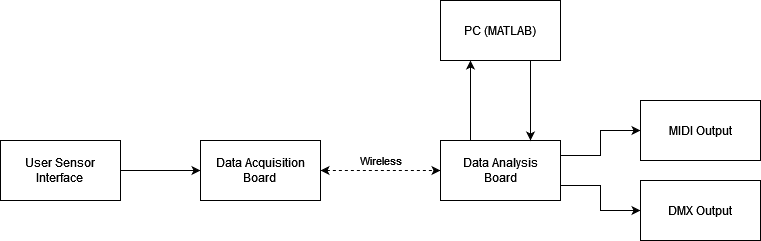
\includegraphics[width=1\columnwidth]{chapters/project_plan/figures/System_Block_Diagram}
\end{figure}

\begin{figure}[!ht]
    \caption{Acquisition flow diagram}\label{fig:acquisition}
    \centering
    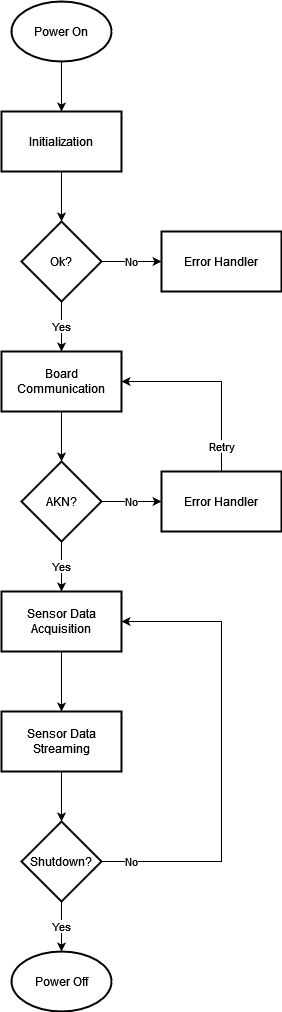
\includegraphics[scale=0.40]{chapters/project_plan/figures/Acquisition_Flow_Diagram}
\end{figure}

\begin{figure}[!ht]
    \caption{Analysis flow diagram}\label{fig:analysis}
    \centering
    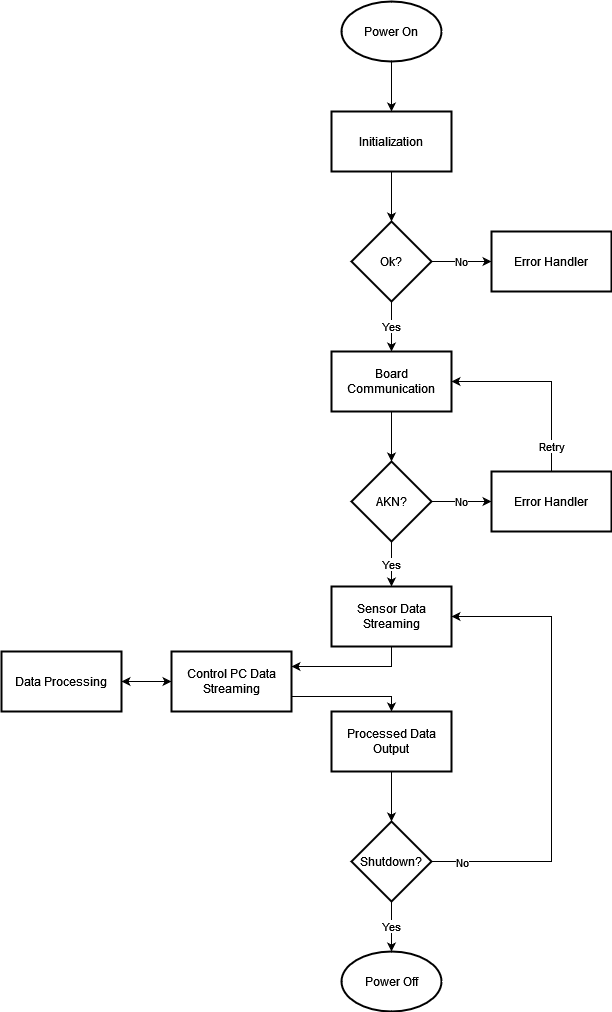
\includegraphics[scale=0.40]{chapters/project_plan/figures/Analysis_Flow_Diagram}
\end{figure}

\section{Methodology}
The methodology employed in this project adheres to a structured approach as depicted in \autoref{fig:methodology}.
The initial step involves defining the project objectives and scope in a meticulous and well-defined manner.
Subsequently, a comprehensive market analysis is performed to identify the gap in the market that the project will fulfill.
Based on the analysis, the project requirements are specified, which outline the essential metrics and benchmarks necessary for the project to succeed.
\\
Once the requirements have been established, various options are analyzed and evaluated to determine the most suitable course of action.
The development and prototyping phase follows, where the system is continuously tested to ascertain its conformity with the established requirements.
If the system fails to meet the requirements, the process repeats,
and the analysis, development, and prototyping are redone until the desired outcome is achieved.
Upon successful testing and meeting the requirements, the project moves into the closing phase,
where the project documentation is compiled and handed over to the client.
This approach ensures that the project is executed in a systematic and organized manner,
leading to the delivery of a high-quality product.

\begin{figure}[!ht]
    \caption{Methodology}\label{fig:methodology}
    \centering
    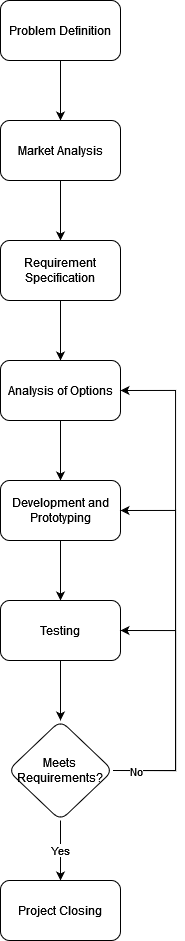
\includegraphics[scale=0.40]{chapters/project_plan/figures/Methodology}
\end{figure}

\section{Data Analysis}
The data analysis methodology that will be employed in this project involves a series of steps
to ensure that the collected data is within its usable frequency and at a reasonable magnitude.
First, the sensors that will be used for data collection will be carefully selected and rigorously tested
using specialized equipment such as an oscilloscope.
The data collected from the sensors will then be analyzed to determine the active frequency range and magnitude.
This analysis will inform the design of appropriate filters and amplifiers to be used in the acquisition board.
\\
Once the filters and amplifiers have been designed, the sensors will again be tested to determine if they correctly interface with the acquisition board.
The largest measured value of the sensor will be used to calibrate the acquisition board,
ensuring that the data collected is at the highest resolution possible without loss of information due to clipping.
This process of analysis, design, and testing will be repeated as necessary
to ensure that the sensor data collected is of the highest quality and meets the project requirements.

\section{Work Plan}
A detailed work plan can be found in \autoref{fig:gantt}.
The work plan has been designed to try and maximise the number of concurrent tasks that can be undertaken.
A high level view of the work plan can be found in \autoref{fig:gantt_high_lvl}.

\begin{figure*}[!ht]
    \caption{High level breakdown of gantt chart}\label{fig:gantt_high_lvl}
    \centering
    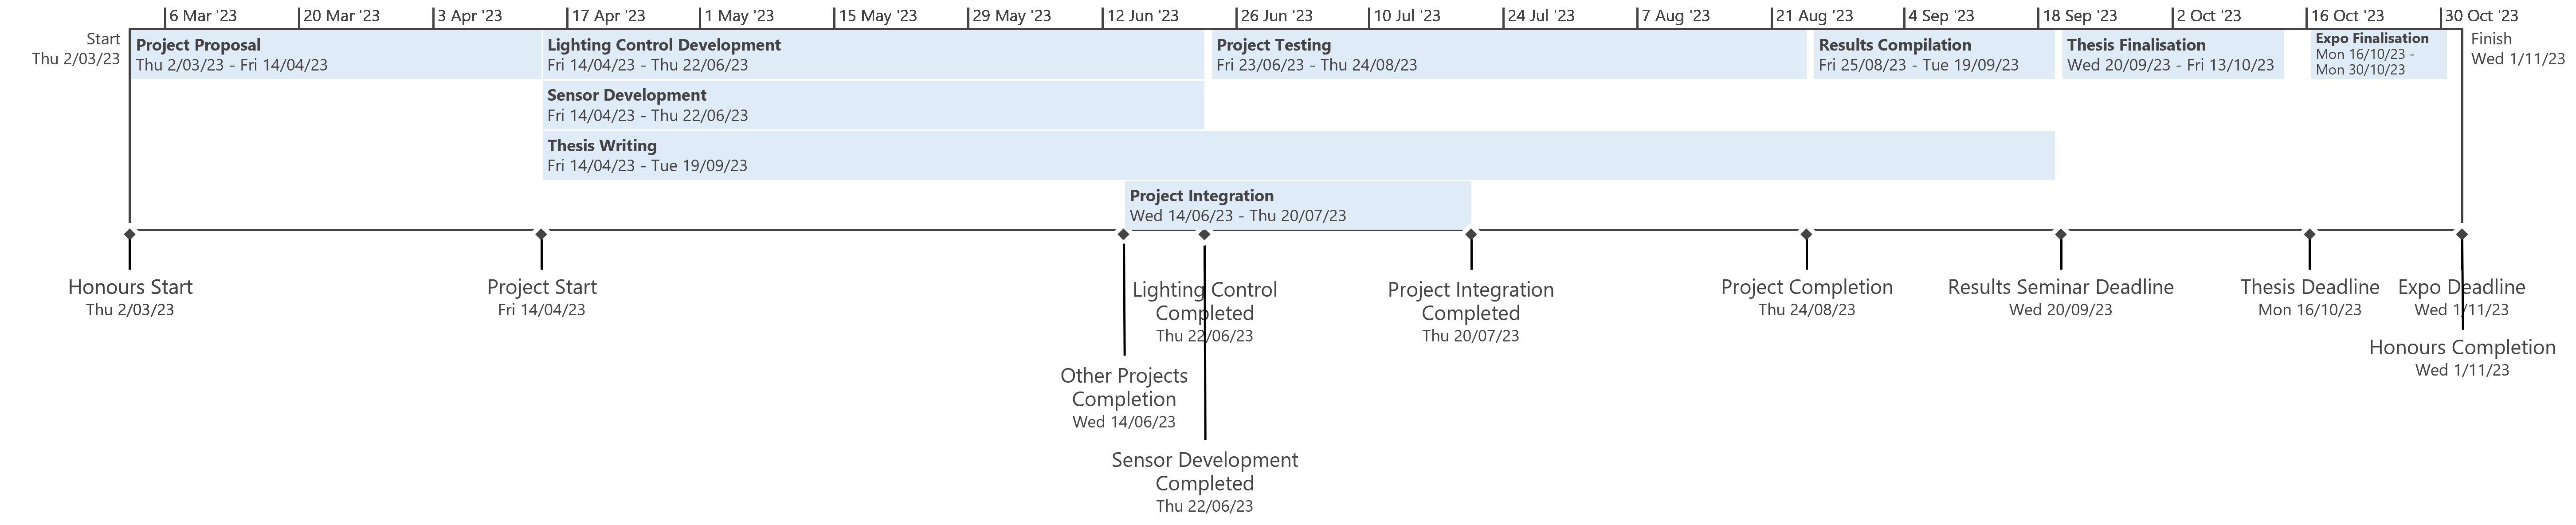
\includegraphics[width=2\columnwidth]{chapters/project_plan/figures/Gantt_Chart_High_Level}
\end{figure*}

\begin{figure*}[!ht]
    \caption{Gantt Chart}\label{fig:gantt}
    \centering
    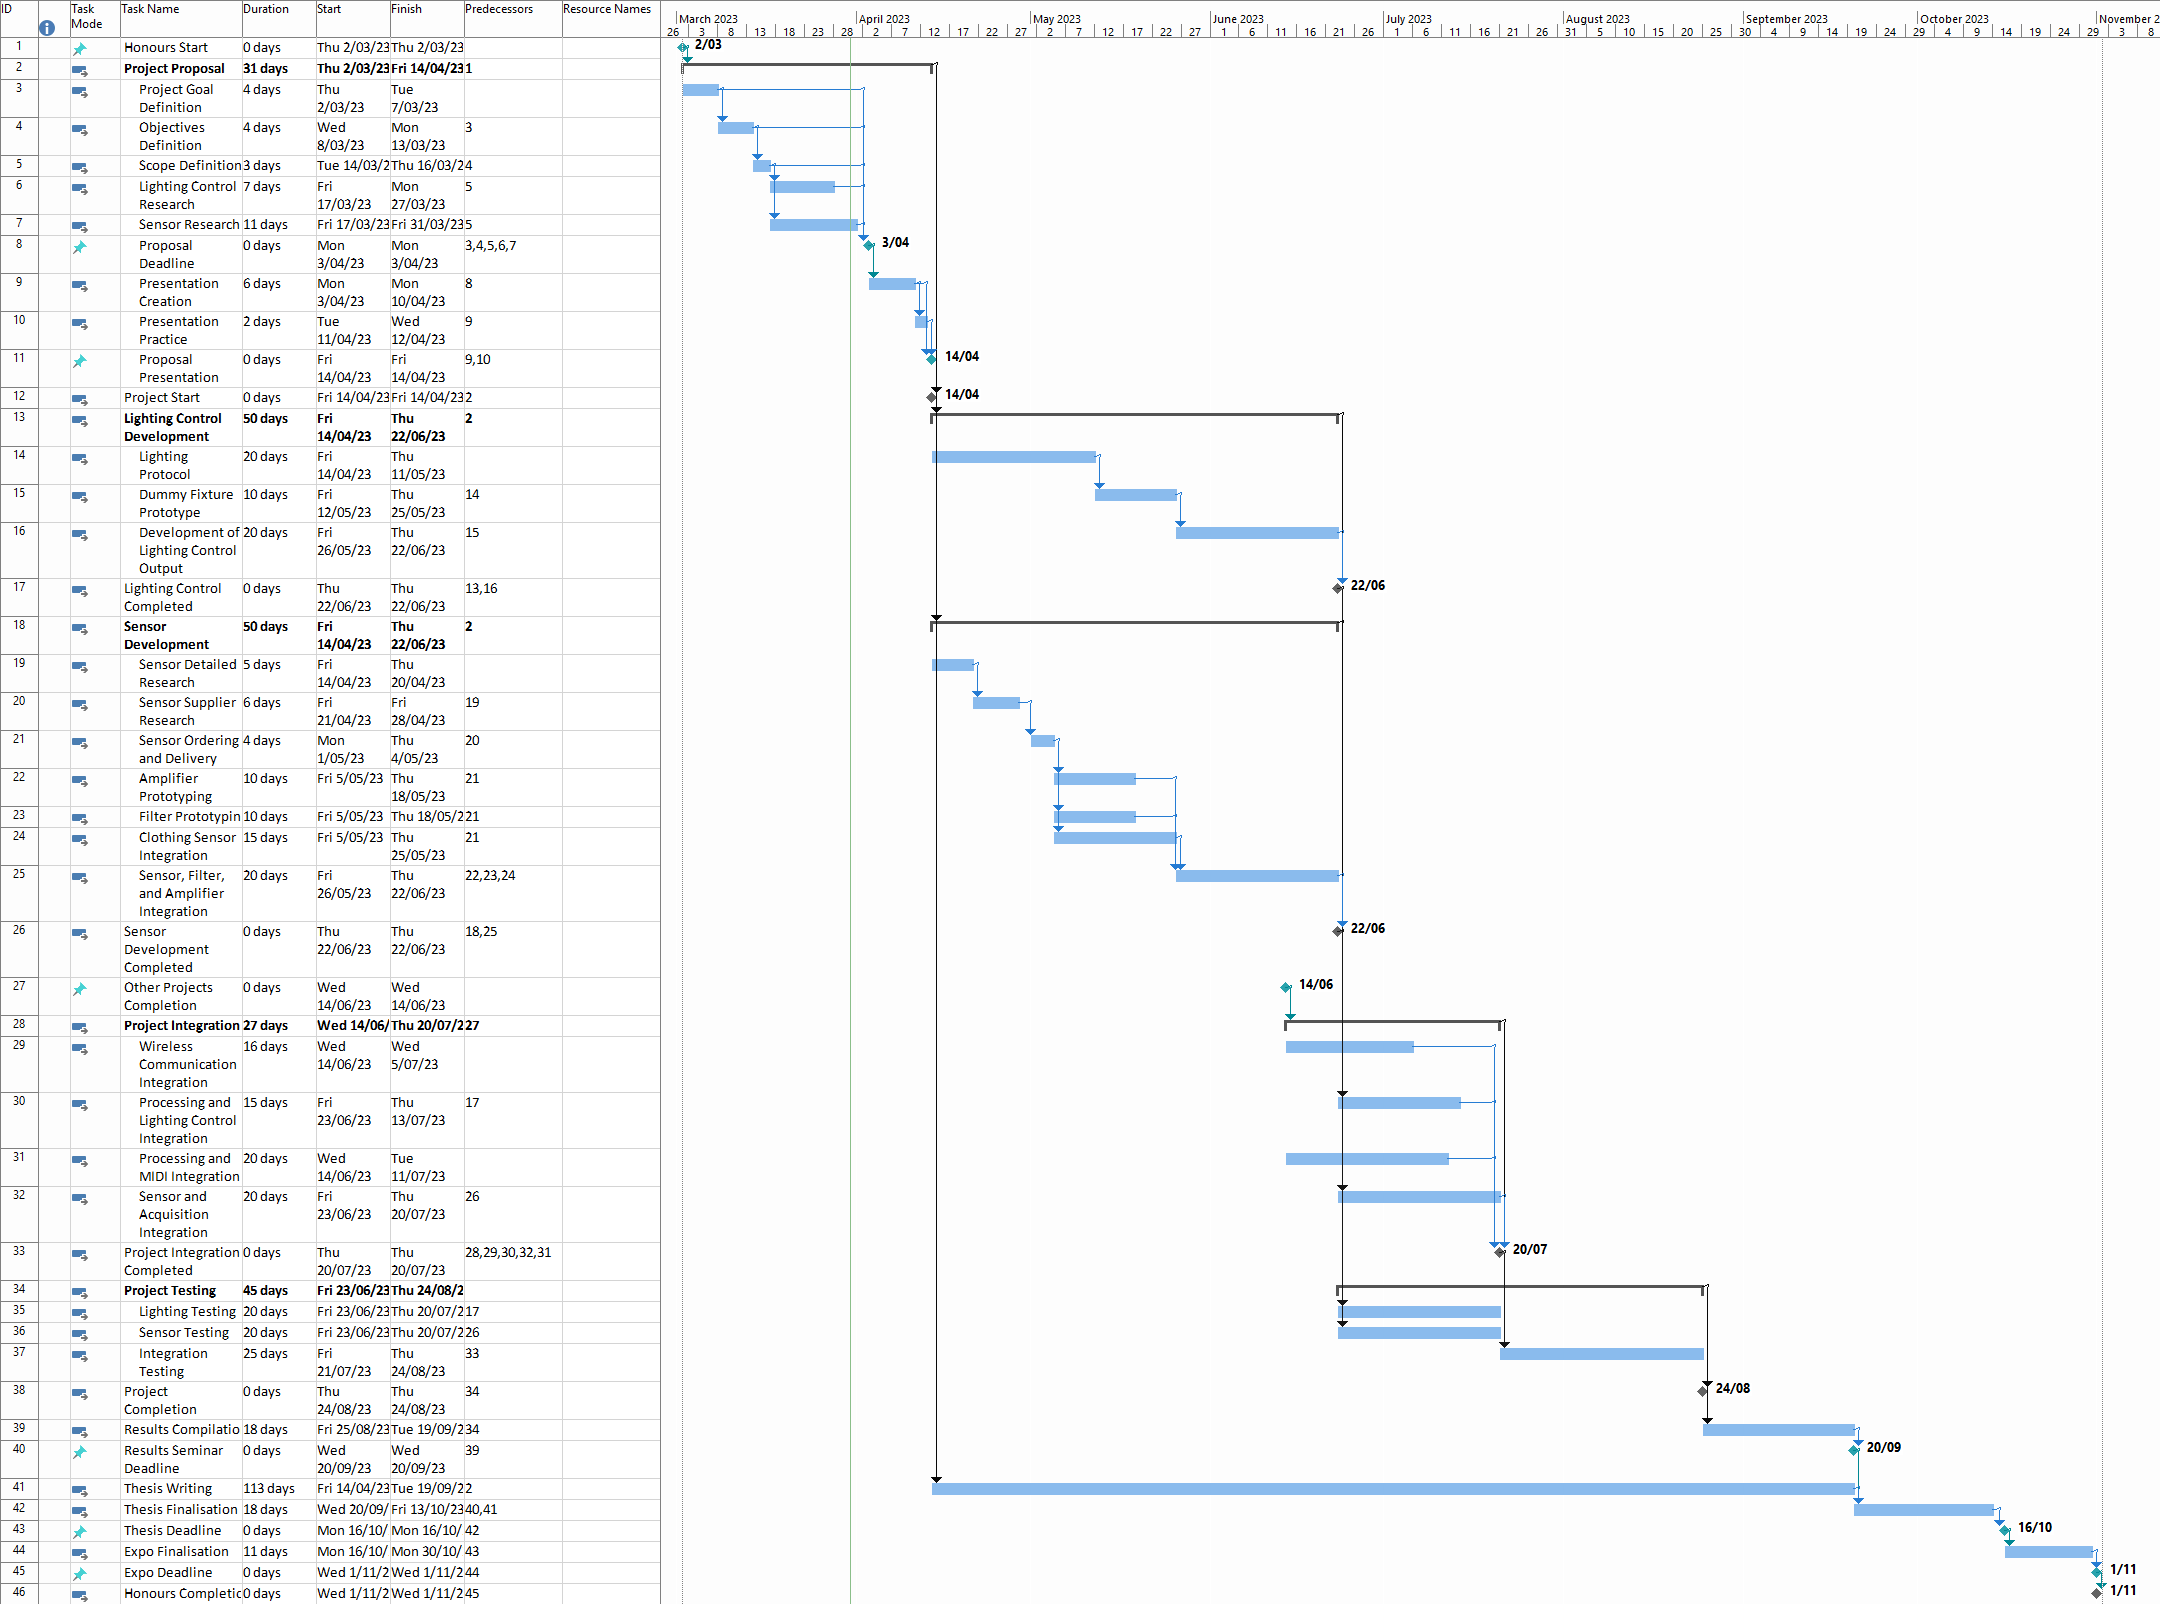
\includegraphics[width=2\columnwidth]{chapters/project_plan/figures/Gantt_Chart}
\end{figure*}

\section{Budget}
The total budget of the project cannot exceed the \$600 constraint.
There are a variety of mechanical biosensors that have already been provided for no cost and thus do not need to be purchased.
Of the sensors that will be bought, they will primarily consist of electrode based bio-sensing.
The quoted budget for these sensors are:

\begin{itemize}
    \item \$8.95 for 10 electrodes,
    \item \$10.95 for 10 electrode cables,
    \item \$30 for fingerprint sensor
    \item \$100 for PCB interfaces
\end{itemize}

For a total of \$149.9.
It is important to note that this is an estimated budget,
there are some potential additional costs since the electrodes only have limited uses.
To allow for this, the budget has been set to \$250.

\section{Risk Management}
There are three risks to the success of this project.

The first risk is the lack of DMX equipment to test project functionality with.
This risk can be mitigated by using simulated hardware.
Since the DMX protocol is very well defined,
dummy DMX fixtures can be made using cheap, off-the-shelf microcontrollers.

Secondly, the other honours projects that are underway and completing at the end of this semester.
As the scope of these projects were set before the beginning of this project,
there is a chance that they could encroach on the scope of the project.
To mitigate this risk, the project has been given stretch goals.
This allows the project scope to still be well defined,
while not limiting the scope of the other projects.

The final risk is that the supply chain for electronic components can cause shortages and delays.
This risk has been mitigated by allowing the project to operate using older hardware,
requiring no new stock to be purchased in the case of a supply chain shortage.
In that case, all new suggestions from this project will be considered for future iterations,
and further development will be made modular enough to allow the changes to be implemented.

\section{Conclusion}
Based on the research and analysis conducted,
we propose the development of a system for providing music and lighting control using biological signals.
This system will improve accessibility for musical performance,
while also providing new exciting possibilities to existing performers through biosensor based lighting control.
